% Felipe Bandeira da Silva

%\documentclass[a4paper, 10pt]{article}
\documentclass[paper=a4, fontsize=11pt]{article}

\usepackage[brazil]{babel}
\usepackage[utf8]{inputenc}
\usepackage{listings}
\usepackage{color}
\usepackage{amsthm}
\usepackage{graphicx}

%\usepackage{schemabloc}
%\usetikzlibrary{circuits}

\setlength{\parindent}{0pt}
\setlength{\parskip}{18pt}

\renewcommand{\labelitemi}{$-$}

\begin{document}


Como já é de conhecimento de todos, os testes feitos no ''formigueiro'' apresentam
resultados estranhos e totalmente incoerentes. Ensaios estes que 
são realizados utilizando os seguintes equipamentos(todos conectados na mesma fonte, 220V):
\begin{itemize}
    \item Fonte Geradora de Alta Tensão(desenvolvida por: LCE, LAMOTRIZ)
\item Sistema de aquisição(Agilent U2535, Sensor de corrente(Hall) e Tensão, Netbook)
\item Osciloscópio(ponteira de alta tensão e ponteira de corrente, usado apenas 
para comparação com o software Labview.
\end{itemize}

Lembrando, os ensaios realizados na Hidráulica e no estacionamento do DEE 
apresentam resultados coerente. O sinal é considerado coerente quando a forma de onda
medida pelos instrumentos, pode ser representada pela equação 1. Equação esta que 
não leva em consideração os efeitos indutivos e capacitivos. 

\begin{equation}
v(t) = V_p e^{-t/\tau}
\end{equation}

Onde $V_p$ representa a tensão de pico da fonte, em torno de $810 V$. A constante
$\tau$ é dependente da resistência de Thevenin vista pela fonte, pontos A e B, mostrados
na figura 1. Para uma resistência de 100 $\Omega$ entre os pontos A e B, considerando
uma capacitância de 1.1 $\mu F$
o circuito 
deve responder de tal forma, que é necessário 550 $\mu s$ para o descarregamento de 
99 $\%$ do capacitor(localizado internamente na fonte).

\begin{figure}[!ht]
    \centering
    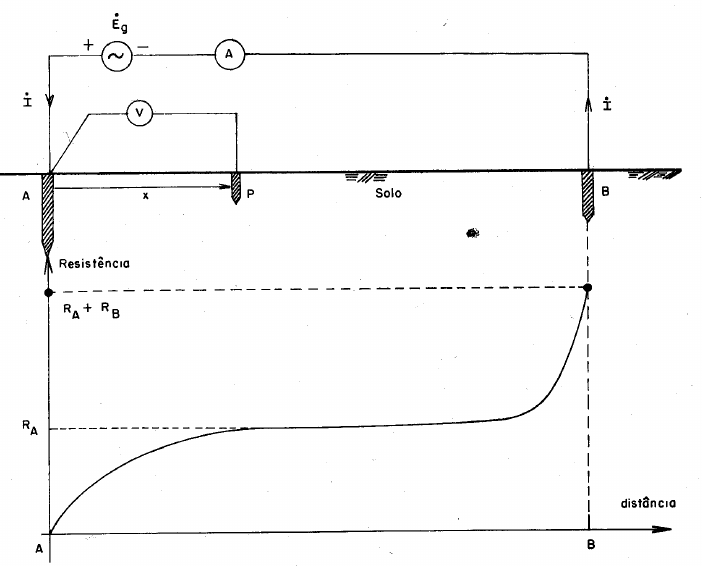
\includegraphics[scale=.4]{medicao.png}
    \caption{Curva de Resistência de Terra x Distância, Fonte: Kinderman}
\end{figure}
Agora o "formigueiro" sempre apresenta ruídos, na tentativa de encontrar o 
problema foram feitos as seguintes ações,

Ação 0, retirar o sistema de aquisição das medições. Deixando apenas o osciloscópio.
Para tanto, foi conectado na saída do Fonte apenas o  dois eletrodos(retorno e topologia)

\end{document}
